\chapter{IT Service Management}
\label{chap: IT Service Management}

\section{Alternativen}
\label{chap: Moeglichkeiten zur Servicedefinierung}

Alle Unternehmen stellen Dienstleistungen zur Verfügung. Doch damit dies auch in angemessener Qualität zustande kommt, 
müssen Unternehmen permanent agil und anpassungsfähig sein. Durch die Definierung der IT-Services, mittels einer Ansetzung an Best Practices, 
ist die Erhöhung der Erfolgschancen deutlich höher.
\

Dabei bieten diese Quellen Best Practices:

\begin{quote}
    \begin{itemize}
        \item   \emph{Öffentliche Frameworks und Standards
        \item   Proprietäres Wissen von Organisation und einzelnen Personen}
    \end{itemize}
\end{quote}

so laut \citetitle[]{ITIL}\footcite[][Kap.\ 1.1, S.\ 1]{ITIL}

\noindent
\\
In diesem Fall entscheiden wir uns in der Projektgruppe für die erste Möglichkeit,
weil innerhalb des Unternehmens SSIT Solutions KG kein qualifiziertes
 Wissen bezüglich des IT Service Managements vorhanden ist.
 Dabei stellt sich nur noch in Frage, welches der Frameworks sich am effizientesten eignet.

\subsection{Vergleich zwischen diversen Frameworks}
\label{chap: Vergleich Frameworks}

Es gibt eine Menge an öffentlichen Frameworks, die von verschiedenen Publikatoren
veröffentlicht wurden. Jedoch sind drei von ihnen in diesem Fall interessant.
Absteigend sortiert nach Häufigkeit der Verwendung:
\\
\begin{itemize}
    \item \textbf{ITIL}:  \textbf{I}nformation \textbf{T}echnology \textbf{I}nfrastructure
                          \textbf{L}ibrary
    \item \textbf{COBIT}: \textbf{C}ontrol \textbf{Ob}jectives for \textbf{I}nformation 
                          and Related \textbf{T}echnologies
    \item \textbf{MOF}:   \textbf{M}icrosoft \textbf{O}perations \textbf{F}ramework
\end{itemize}
\noindent
\\
Zwar sind alle Frameworks effizient, doch erst wenn sie in der richtigen
Ausgangslage verwendet werden. 
\\
Hier eine kurze Darstellung der Kernprozesse der erwähnten Frameworks:

\begin{itemize}
    \item ITIL
    \begin{itemize}
        \item Service Strategy
        \item Service Design
        \item Service Transition
        \item Service Operation
        \item Continual Service Improvement
    \end{itemize}
    \item COBIT
    \begin{itemize}
        \item Plan and Organise
        \item Acquire and Implement
        \item Deliver and Support
        \item Monitor and Evaluate
    \end{itemize}
    \item MOF
    \begin{itemize}
        \item Plan
        \item Deliver
        \item Operate
        \item Manage
    \end{itemize}
\end{itemize}

\noindent
\\
COBIT wird eher für Unternehmen verwendet, die hauptsächlich
 eine Prüfung der IT-Prozesse durchführen. Darin ist dieses Framework mit ITIL zwar ziemlich
 ähnlich, aber der Hauptunterschied liegt dabei, dass COBIT prozessbasiert ist.
 ITIL hingegen ist dienstleistungsbasiert.{\footnote{\url{https://de.wikipedia.org/wiki/COBIT}}
\\
MOF ist verglichen mit ITIL allerdings basierend auf Service Management Funktionen
und geeignet für alltägliche IT Praktiken, wobei beide einem Lebenszyklus 
der Dienstleistungen folgen.\footnote{\url{https://technet.microsoft.com/en-us/library/dd320379.aspx}}
\\
Doch aufgrund der weltweiten Verbreitung und Bekanntheit von ITIL, wurde in der Projektgruppe 
dieses Framework als IT Service Management ausgewählt. Auch unser Abteilungsvorstand Dipl.-Ing 
Felix Schwab hat uns ITIL empfohlen. Somit stand dies fest.

\section{Allgemeines über ITIL}
\label{chap: ITIL im Detail}


\subsection{Wie kann man erfolgreich sein?}
Damit man mittels ITIL erfolgreich sein kann, beziehen sich Unternehmer auf die vorteilreichen Beschreibungen von Praktiken,
um mit diesen einen Return on Investment (Ertrag einer Investition) zu erzielen. Dadurch können Organisationen beispielsweise 
Folgendes erlangen:


\begin{quote}
\begin{itemize}
    \item \emph{Schaffung von Mehrwert für Kunden durch Services durch verbesserte Kundenbeziehungen
    \item Integration der Geschäftsstrategie sowie der Bedürfnisse des Kunden in die Strategien von Services
    \item Messung, Überwachung und Optimierung der Leistung von IT Services und Service Provider und Senkung von Kosten}
    \footcite[][Kap.\ 1.2, S.\ 2]{ITIL}
    \item uvm.
\end{itemize}
\end{quote}

\subsection{Servicelebenszyklus}
\label{chap: Servicelebenszyklus}
\noindent
Seit mehr als zwei Jahrzenten ist ITIL erfolgreich eingesetzt worden. Im Laufe dieser Zeitspanne hat sich das Framework immer mehr
weiterentwickelt und stellt sich nun als ein prozessbasiertes Framework mit einer vollständigen Sicht auf den Servicelebenszyklus.
\\
\noindent
\\
\begin{tabular}{l|p{10cm}}
    \textbf{Servicelebenszyklus} & Koordination und Steuerung der Funktionen, Prozesse und Systeme, die für das Management des gesamten 
    Lebenszyklus von IT Services notwendig sind. Darunter versteht man die Kernbereiche Strategie, Design, Transition, Betrieb und die kontinuierliche
    Verbesserung von IT Services. Auch bekannt unter Service Management Lebenszyklus.
\end{tabular}

\begin{figure}[H]
    \centering
    \captionsetup{justification=centering,margin=2cm}
    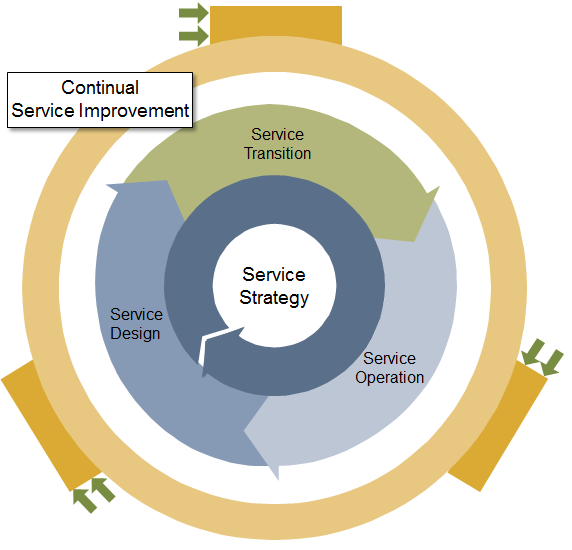
\includegraphics[scale=0.5]{images/ITIL/servicelebenszyklus}
    \caption[Servicelebenszyklus laut ITIL]{Servicelebenszyklus laut ITIL, Quelle\footnotemark}
\end{figure}

\footnotetext{Quelle: \url{https://www.glenfis.ch/custom/FoundationDemo/index.html?sm_servicelebenszyklus.htm}}

\subsection{Service Management}
\label{chap: Service Management}

Um das Service Management erklären zu können, muss man wissen was ein Service ist.
Die Definition wäre folgendermaßen:
\\\\

\begin{tabular}{l|p{10cm}}
    \textbf{Service} & Mittel für die Bereitstellung von Mehrwerten für Kunden mit Befreiung der Kunden von spezifischen Kosten und Risiken.
\end{tabular}
\\ \\
\emph{Services unterstützen Ergebnisse, indem die Ausführung von zugehörigen Aufgaben verbessert und die Auswirkungen möglicher Einschränkungen verringert werden.}
\citetitle[]{ITIL}\footcite[][Kap.\ 1.3, S.\ 6]{ITIL}
\\ \\
Hier versteht man unter Einschränkungen zum Beispiel finanzielle oder technologische Hindernisse.
Doch nicht nur solches, sondern auch Vorschriften seitens der Kunden. 
\\
Dabei unterscheidet man drei Arten von Services:

\begin{tabular}{l | p{10cm}}
    \textbf{Core Services} & Diese dienen dazu, um die erforderlichen Ergebnisse von bis zu mehreren Kunden zu erzielen. \\ \\
    \textbf{Enabling Services} & Solche sind dafür da, um überhaupt Core Services zu ermöglichen. Ohne \emph{Enabling Services} sind Core Services nicht von Nützen. \\ \\
    \textbf{Erweiternde Services} & Sind Services, die man im Prinzip nicht braucht, die aber zu einem Core Service hinzugefügt werden können, um ihn für den Kunden verlockend interessant darzustellen.
\end{tabular}
\leavevmode
\\ \\
Service Providern wird es ermöglicht durch das Service Management, die Services die er zur Verfügung stellt, zu verstehen.
Anhand des Service Managements kann man sich vergewissern, dass die Services die Ergebnisse liefern, die man auch tatsächlich erreichen möchte.
Somit kann man auch Risiken und Kosten, durch das Bewusstsein des jetzigen Zustandes eines Services, verstehen und verhindern oder sogar erwarten und durch Work-Arounds lösen.
\\ \\
Also kann man das Service Management so definieren:
\\ \\
\begin{tabular}{l | p{10cm}}
    \textbf{Service Management} & Zurverfügungstellung von Mehrwert durch koordinierte, spezialisierte und organisatorische Fähigkeiten als Services.
\end{tabular}
\\ \\
Solche Fähigkeiten, die die Strukturierung und Verwirklichung mittels Services ermöglichen, kann man darstellen als Prozesse, Rollen, Funktionen und Aktivitäten.
\\ \\
Jedoch reichen allein diese Fähigkeiten nicht aus, um das Ziel zu erreichen. Man muss sich im Klaren sein, wie man diese Fähigkeiten zielgerecht einsetzt -
Dies bedarf an Wissen und Verständnis, sowie der Auseinandersetzung mit den einzelnen Elementen.
\\ \\
Das Service Management kümmert sich um jede Komponente, denn jede Komponente verfügt über einen Lebenszyklus und das Service Management beachtet den vollständigen Lebenszyklus.

\subsection{Prozesse und Funktionen}
\label{chap: Prozesse und Funktionen}

Ein Prozess beinhaltet eine Reihe an Aktivitäten, um ein fixes Ziel zu erreichen. Es können mehrere Inputs in definierte Outputs umgewandelt werden. Diese Ergebnislieferung kann durch Rollen, Verantwortlichkeiten, 
Hilfsmittel und noch durch andere Möglichkeiten unterstützt oder eingeschränkt werden.
\\ \\
Merkmale von Prozessen sind:
\begin{itemize}
    \item Messbarkeit
    \item Identifizierbarkeit
    \item Existenz für Ergebnislieferung
    \item Reaktion und Handlung auf bestimmte Ereignisse
\end{itemize}

\leavevmode
\\
Unter einer Funktion hingegen versteht man eine Zusammensetzung von mehreren Personen mit Hilfsmitteln und Ressourcen, um Prozesse oder Aktivitäten durchzuführen.
\\
Solchen Teams kann man Verantwortlichkeiten zuweisen. Diese nennt man Rollen.

\subsection{Rollen}
\label{chap: Rollen}

\emph{Eine Rolle ist ein Satz von Verantwortlichkeiten, Aktivitäten und Kompetenzen, die einer Person oder einem Team zugewiesen sind.}
\citetitle[]{ITIL}\footcite[][Kap.\ 1.5, S.\ 12]{ITIL}
\\ \\
\underline{Einige Rollen innerhalb des ITIL Frameworks:}
\\ \\
\begin{tabular}{l|p{10cm}}
    \textbf{Process Owner} & Der \emph{Process Owner} ist dafür zuständig, dass die Existenz der Ergebnislieferung im richtigen Ausmaß und nach vereinbarten Standards innerhalb von Dokumentationen verläuft. \\ \\
    \textbf{Process Manager} & Der \emph{Process Manager} ist für das operative Management zuständig. Darunter versteht man die Rollenzuweisung der Mitarbeiter, das Managen der Ressourcen, Monitoring und Reporting des Prozesszustands, 
    aber auch durch das Bewusstsein der Situation, das Durchführen von Verbesserungen. \\ \\
    \textbf{Process Practitioner} & Der \emph{Process Practitioner} durchführt mindestens eine Aktivität innerhalb des Prozesses und kontrolliert ob die Inputs sowie die Outputs in Ordnung sind. \\ \\
    \textbf{Service Owner} & Der \emph{Service Owner} ist verantwortlich für die Erbringung und für die Wartung eines Services.
\end{tabular}

\section{Service Strategy Implementierung}
\label{chap: SS Implementierung}

\subsection{Zweck und Ziel}
\label{chap: Zweck und Ziel}

In diesem Kapitel ist es wichtig die Herangehensweise zu definieren, um die geschäftlichen Ziele
erreichen zu können. 
\\
Dafür existieren innerhalb der Service Strategy die \emph{vier Ps}, damit ein Service Provider die Ziele ermöglichen kann.
Diese sollen als Anhaltspunkt und als Hilfsmittel über den momentanen Zustand und die Richtung helfen.
\\
Dabei versteht man unter den vier Ps diese Aspekte:
\\
\begin{itemize}
    \item Perspective
    \item Position
    \item Plan
    \item Pattern
\end{itemize}

\noindent
\\
Durch das Bewusstsein von diesen vier P's der Service Strategy, erlangt man den richtigen Weg gen Ziel.

\subsubsection{Perspective}
\label{chap: Perspective}

Bei der Bestimmung der Perspektive muss man die Richtung, die Werte, die Vorstellungen und den Zweck definieren.
\\
In diesem konkreten Fall der Diplomarbeit, ist es dabei wichtig ob die Endgeräte der Kunden in einem kritischen Zustand
sind oder nicht. Darunter wär also zu verstehen dass die 
\begin{labeling}{Vorstellungen}
    \item [Richtung] das Monitoring ist.
    \item [Werte] die Endgeräte selbst sind.
    \item [Vorstellungen] die Statusse der Endgeräte im grünen Bereich erfolgen.
    \item [Zwecke] die Zufriedenheit der Kunden sind.
\end{labeling}

\subsubsection{Position}
\label{chap: Position}

In diesem Bereich der vier Ps der Service Strategy ist es wichtig, die Unterschiede zwischen anderen Wettbewerben zu erkennen zu geben.
\\
Solch wichtige Informationen können den Kunden die Relevanz zeigen und dem Unternehmen somit einen Kunden gewinnen.
\\
Denn ein Unternehmen mit einer definierten Position, informiert die Kunden über die Einzigartigkeit gegenüber anderen Unternehmen.
\\
Natürlich kann es auch andere Unternehmen geben, die Icinga verwenden, aber in unserem Fall spezialisieren wir Icinga und adaptieren dieses
nutzvolle, große System an unseren Auftraggeber und ermöglichen ihm die angenehme Überwachung von Kundennetzwerken.
\\\\
Die Position der SSIT Solutions KG, im konkreten Fall Icinga, ist also das Überwachen der Kundennetzwerke ohne dass ein Techniker zu diesem Kunden
rüberfahren muss um gewisse Details zu erfahren. Bis jetzt war dies so und nun wird das verbessert. Dies wird angenehm von den derzeitigen Kunden betrachtet
und wie erwähnt, mit hoher Wahrscheinlichkeit noch mehr Kunden dazu bringen Dienstleistungen von diesem Unternehmen zu verwenden.

\subsubsection{Plan}
\label{chap: Plan}

Dabei ist es wichtig zu wissen, \underline{wie} man dies erreicht. 
\begin{enumerate}
    \item Es wird ein Icingaserver zur Verfügung gestellt.
    \item Man muss am Anfang mindestens einmal zum Kunden fahren, um Gerätedaten zu extrahieren (IP innerhalb des Netzwerks).
    \item Die Kundennetzwerke werden mit dem Server verbunden.
    \item Es werden Überwachungen durch diesen Server bereitgestellt durch die vorhandene CSV Datei mit Gerätedaten, die man nur noch importieren muss.
\end{enumerate}

\subsubsection{Pattern}
\label{chap: Muster}

Damit das Monitoring und der ganze Sinn und Zweck dieser Diplomarbeit auch reibungslos funktionieren kann, definiert man Vorlagen für die Herangehensweise der Musterlösungen.
\\
Eine Möglichkeit wäre, die Statusse der Netzwerke in einem bestimmten Intervall abzufragen.
\\
Konkretes Beispiel - Pingabfrage:

% Hier folgt dann ein Muster mit einem Screenshot für eine Pingabfrage 

\subsection{Service Design Implementierung}
\label{chap: SD Implementierung}

